\documentclass[11pt,dvipsnames,usenames,aspectratio=169]{beamer}  % Add handout to options to disable overlays

% For more themes, color themes and font themes, see:
% http://deic.uab.es/~iblanes/beamer_gallery/index_by_theme.html
%
\mode<presentation>
{%
  \usetheme{CambridgeUS}    % or try default, Darmstadt, Warsaw, ...
  \usecolortheme{whale}     % or try albatross, beaver, crane, ...
  \usefonttheme{serif}          % or try default, structurebold, ...
  % \usefonttheme[onlymath]{serif}
  % \setbeamertemplate{navigation symbols}{}
  % \setbeamercovered{transparent}

  \setbeamercolor{title}{fg=white}
  \setbeamerfont{title}{series=\bfseries}
  \setbeamercolor{frametitle}{fg=black}
  \setbeamerfont{frametitle}{series=\bfseries}

  \setbeamercolor{section in head/foot}{fg=white}
  \setbeamerfont{section in head/foot}{series=\bfseries}
  \setbeamercolor{subsection in head/foot}{fg=white}
  \setbeamerfont{subsection in head/foot}{series=\bfseries}
  \setbeamercolor{author in head/foot}{fg=white}
  \setbeamerfont{author in head/foot}{series=\bfseries}
  \setbeamercolor{title in head/foot}{fg=white}
  \setbeamerfont{title in head/foot}{series=\bfseries}

  \setbeamercolor{block title}{use=structure,fg=white,bg=title in head/foot.bg}
  \setbeamerfont{block title}{series=\bfseries}
  \setbeamercolor{block body}{use=structure,fg=black,bg=black!1!white}
}

% Support graying out frame elements
\newcommand{\FrameOpaque}{\setbeamercovered{again covered={\opaqueness<1->{40}}}}
% Transition slide
\newcommand{\transitionFrame}[1]{%
{%
  \begin{frame}[plain,noframenumbering]{}{} % the plain option removes the sidebar and header from the title page
    \setbeamertemplate{final page}[text]{\Large \textbf{#1}}
    \usebeamertemplate{final page}
  \end{frame}}
}

\usepackage{fontawesome}  % Used for defining the external hyperlink

% Imported via UltiSnips
\usepackage{graphicx} % Loading the package
\graphicspath{{img/}} % Setting the default folder containing the graphics

\usepackage[makeroom]{cancel}
\renewcommand{\CancelColor}{\color{red}}
\newcommand<>{\xxcancel}[1]{\alt#2{\xcancel{#1}\vphantom{#1}}{#1}}

\usepackage[numbers]{natbib}
\usepackage{appendixnumberbeamer}

% \hypersetup{colorlinks=true,allcolors=blue}

% Here's where the presentation starts, with the info for the title slide
\title[Anchors]{Anchors: High-Precision Model-Agnostic Explanations}
\author[Ribeiro et al.]{%
  {Marco Tulio Ribeiro}\inst{1}
  \and
  {Sameer Singh}\inst{2}
  \and
  {Carlos Guestrin}\inst{1}
}

\institute[UW \& UCI]{%
  \textsuperscript{1}\textbf{University of Washington}
  \and
  \textsuperscript{2}\textbf{University of California, Irvine}
}
\date{November~12, 2020}

% Imported via UltiSnips
\newcommand{\etal}{~et~al.}

% Used for including standalone docs
\usepackage{standalone}

% Imported via UltiSnips
% Unbreakable dash:
%  Words hyphened with these dashes can also be broken at other positions than the dash
%    \-/ hyphen
%    \-- en-dash
%    \--- em-dash
%    extdash unbreakable dashes
%
%  No line breaks possible at the hyphen
%    \=/ hyphen
%    \== en-dash
%    \=== em-dash
\usepackage[shortcuts]{extdash}

% Imported via UltiSnips
% \usepackage{xcolor}
\newcommand{\colortext}[2]{{\color{#1} #2}}
\newcommand{\red}[1]{\colortext{red}{#1}}
\newcommand{\blue}[1]{\colortext{blue}{#1}}
\newcommand{\green}[1]{\colortext{ForestGreen}{#1}}

% Imported via UltiSnips
\usepackage{amsmath}
\DeclareMathOperator*{\argmax}{arg\,max}
\DeclareMathOperator*{\argmin}{arg\,min}
\usepackage{amsfonts}  % Used for \mathbb and \mathcal
\usepackage{amssymb}

% Imported via UltiSnips
\usepackage{mathtools} % for "\DeclarePairedDelimiter" macro
% \swapifbranches changes unstarred paired delimiters to starred and
% vice versa.  This means by default, paired delimiters have the star.
\usepackage{etoolbox}
\newcommand\swapifbranches[3]{#1{#3}{#2}}
\makeatletter
\MHInternalSyntaxOn
\patchcmd{\DeclarePairedDelimiter}{\@ifstar}{\swapifbranches\@ifstar}{}{}
\MHInternalSyntaxOff
\makeatother
% Place after swap to ensure swap star
\DeclarePairedDelimiter{\sbrack}{\lbrack}{\rbrack}
\DeclarePairedDelimiter{\floor}{\lfloor}{\rfloor}
\DeclarePairedDelimiter{\ceil}{\lceil}{\rceil}
\DeclarePairedDelimiter{\abs}{\lvert}{\rvert}
\DeclarePairedDelimiter{\round}{\lfloor}{\rceil}
\DeclarePairedDelimiter{\norm}{\lVert}{\rVert}
\usepackage{bm}
\DeclarePairedDelimiterX\set[1]\lbrace\rbrace{#1}
\DeclarePairedDelimiterX\setbuild[2]\lbrace\rbrace{#1 \bm: #2}
\newcommand{\setint}[1]{{\sbrack{#1}}}
\newcommand{\func}[3]{{#1:#2\rightarrow#3}}
% \newcommand{\defeq}{\stackrel{\mathclap{\mbox{\tiny def}}}{=}}
\newcommand{\defeq}{\coloneqq}
\newcommand{\fedeq}{\eqqcolon}
\newcommand{\expect}[1]{\mathbb{E}\sbrack{#1}}
% Expectation with the subscript defining the distribution
\newcommand{\expectS}[2]{\mathbb{E}_{#1}\sbrack{#2}}

% Allow numbering in align*
\newcommand{\numberthis}{\addtocounter{equation}{1}\tag{\theequation}}

\newcommand{\ints}{\mathbb{Z}}
\newcommand{\intsNN}{\mathbb{Z}_{+}}
\newcommand{\nats}{\mathbb{N}}
\newcommand{\real}{\mathbb{R}}
\newcommand{\realnn}{\real_{{\geq}0}}  % Set of non-negative real numbers

\newcommand{\iidsim}{\stackrel{\mathclap{\mbox{\tiny \textnormal{i.i.d.}}}}{\sim}}

\newcommand{\normaldist}[2]{{\mathcal{N}\mathopen{}\left(#1,#2\right)\mathclose{}}}

% Imported via UltiSnips
\usepackage{array}  % Provides a way add a \centering command to a p-column
\usepackage{arydshln}  % Introduces hdashline & cdashline
\usepackage{bigdelim}
\usepackage{booktabs}
\usepackage{multirow}
\usepackage{makecell}  % Needed for multirowcell

% % Imported via UltiSnips
\usepackage{amsthm}
% \newtheorem{theorem}{Theorem}
% \newtheorem{corollary}{Corollary}[theorem]  % Corollary number derives from theorem
% \newtheorem{lemma}[theorem]{Lemma}  % Lemma and theorem share same counter
% \newtheorem{claim}[theorem]{Claim}  % Same numbering as lemma and theorem
% \newtheorem*{remark}{Remark}
% \newtheorem*{note}{Note}
% \newtheoremstyle{definition}  % <name>
% {3pt}   % <Space above>
% {3pt}   % <Space below>
% % {\itshape}     % <Body font>
% {\normalfont}   % <Body font>
% {}      % <Indent amount>
% {\bfseries} % <Theorem head font>
% {:}     % <Punctuation after theorem head>
% {.5em}  % <Space after theorem head>
% {}      % <Theorem head spec (can be left empty, meaning `normal')>
% \theoremstyle{definition}
% \newtheorem{definition}{Def.}[section]

% Imported via UltiSnips
\usepackage{tikz}
\usetikzlibrary{arrows,decorations.markings,shadows,positioning,calc,backgrounds,shapes}

\usepackage{pgfplots}
\pgfplotsset{compat=1.13}
\usepackage{pgfplotstable}
% \usepackage{subcaption}  % Cannot be used with subfigure

% Handle empty parameters
\usepackage{xifthen}
\newcommand{\ifempty}[3]{%
  \ifthenelse{\isempty{#1}}{#2}{#3}%
}

\newcommand{\dec}{f}
\newcommand{\domainX}{X}
\newcommand{\domainY}{Y}

\newcommand{\X}{x}

\newcommand{\dist}{\mathcal{D}}

\newcommand{\Rule}{A}
\newcommand{\setRule}{\mathcal{A}}
\newcommand{\predicate}{a}

\newcommand{\Prec}[1]{{\text{prec}(#1)}}
\newcommand{\minPrec}{\tau}

\newcommand{\cov}[1]{{\text{cov}(#1)}}
\newcommand{\minCov}{c}

\newcommand{\beamWidth}{B}


% Enable (uncolored) cross-reference hyperlinks
% Should always be last package loaded.
% See: https://tex.stackexchange.com/questions/103123/links-do-not-lead-to-right-pages
\usepackage{hyperref}
\let\oldhref\href
\renewcommand{\href}[2]{\oldhref{#1}{#2\hspace{0.05cm}{\scriptsize\faExternalLink}}}

\begin{document}

\begin{frame}
  \titlepage
\end{frame}

\section{On Rules of Thumb}

\begin{frame}[noframenumbering]{``If silence be good for the wise, how much better for fools.''}
  It takes quite a fool to quote one's self\ldots

  \vspace{25pt}
  \onslide<2->{You're in luck that I am just such a fool...}
\end{frame}

\begin{frame}{SAT'2018 Paper}
  Roughly speaking, the end result is a sampler for which one can largely \\ use the following \green{rule of thumb}:

  \vspace{20pt}
  \begin{center}
    Generating 1,000 perfectly uniform models takes \\
    about 10 times as long as it takes to count the models.
  \end{center}
\end{frame}

\begin{frame}{Week 2 Presentation}
  \begin{center}
    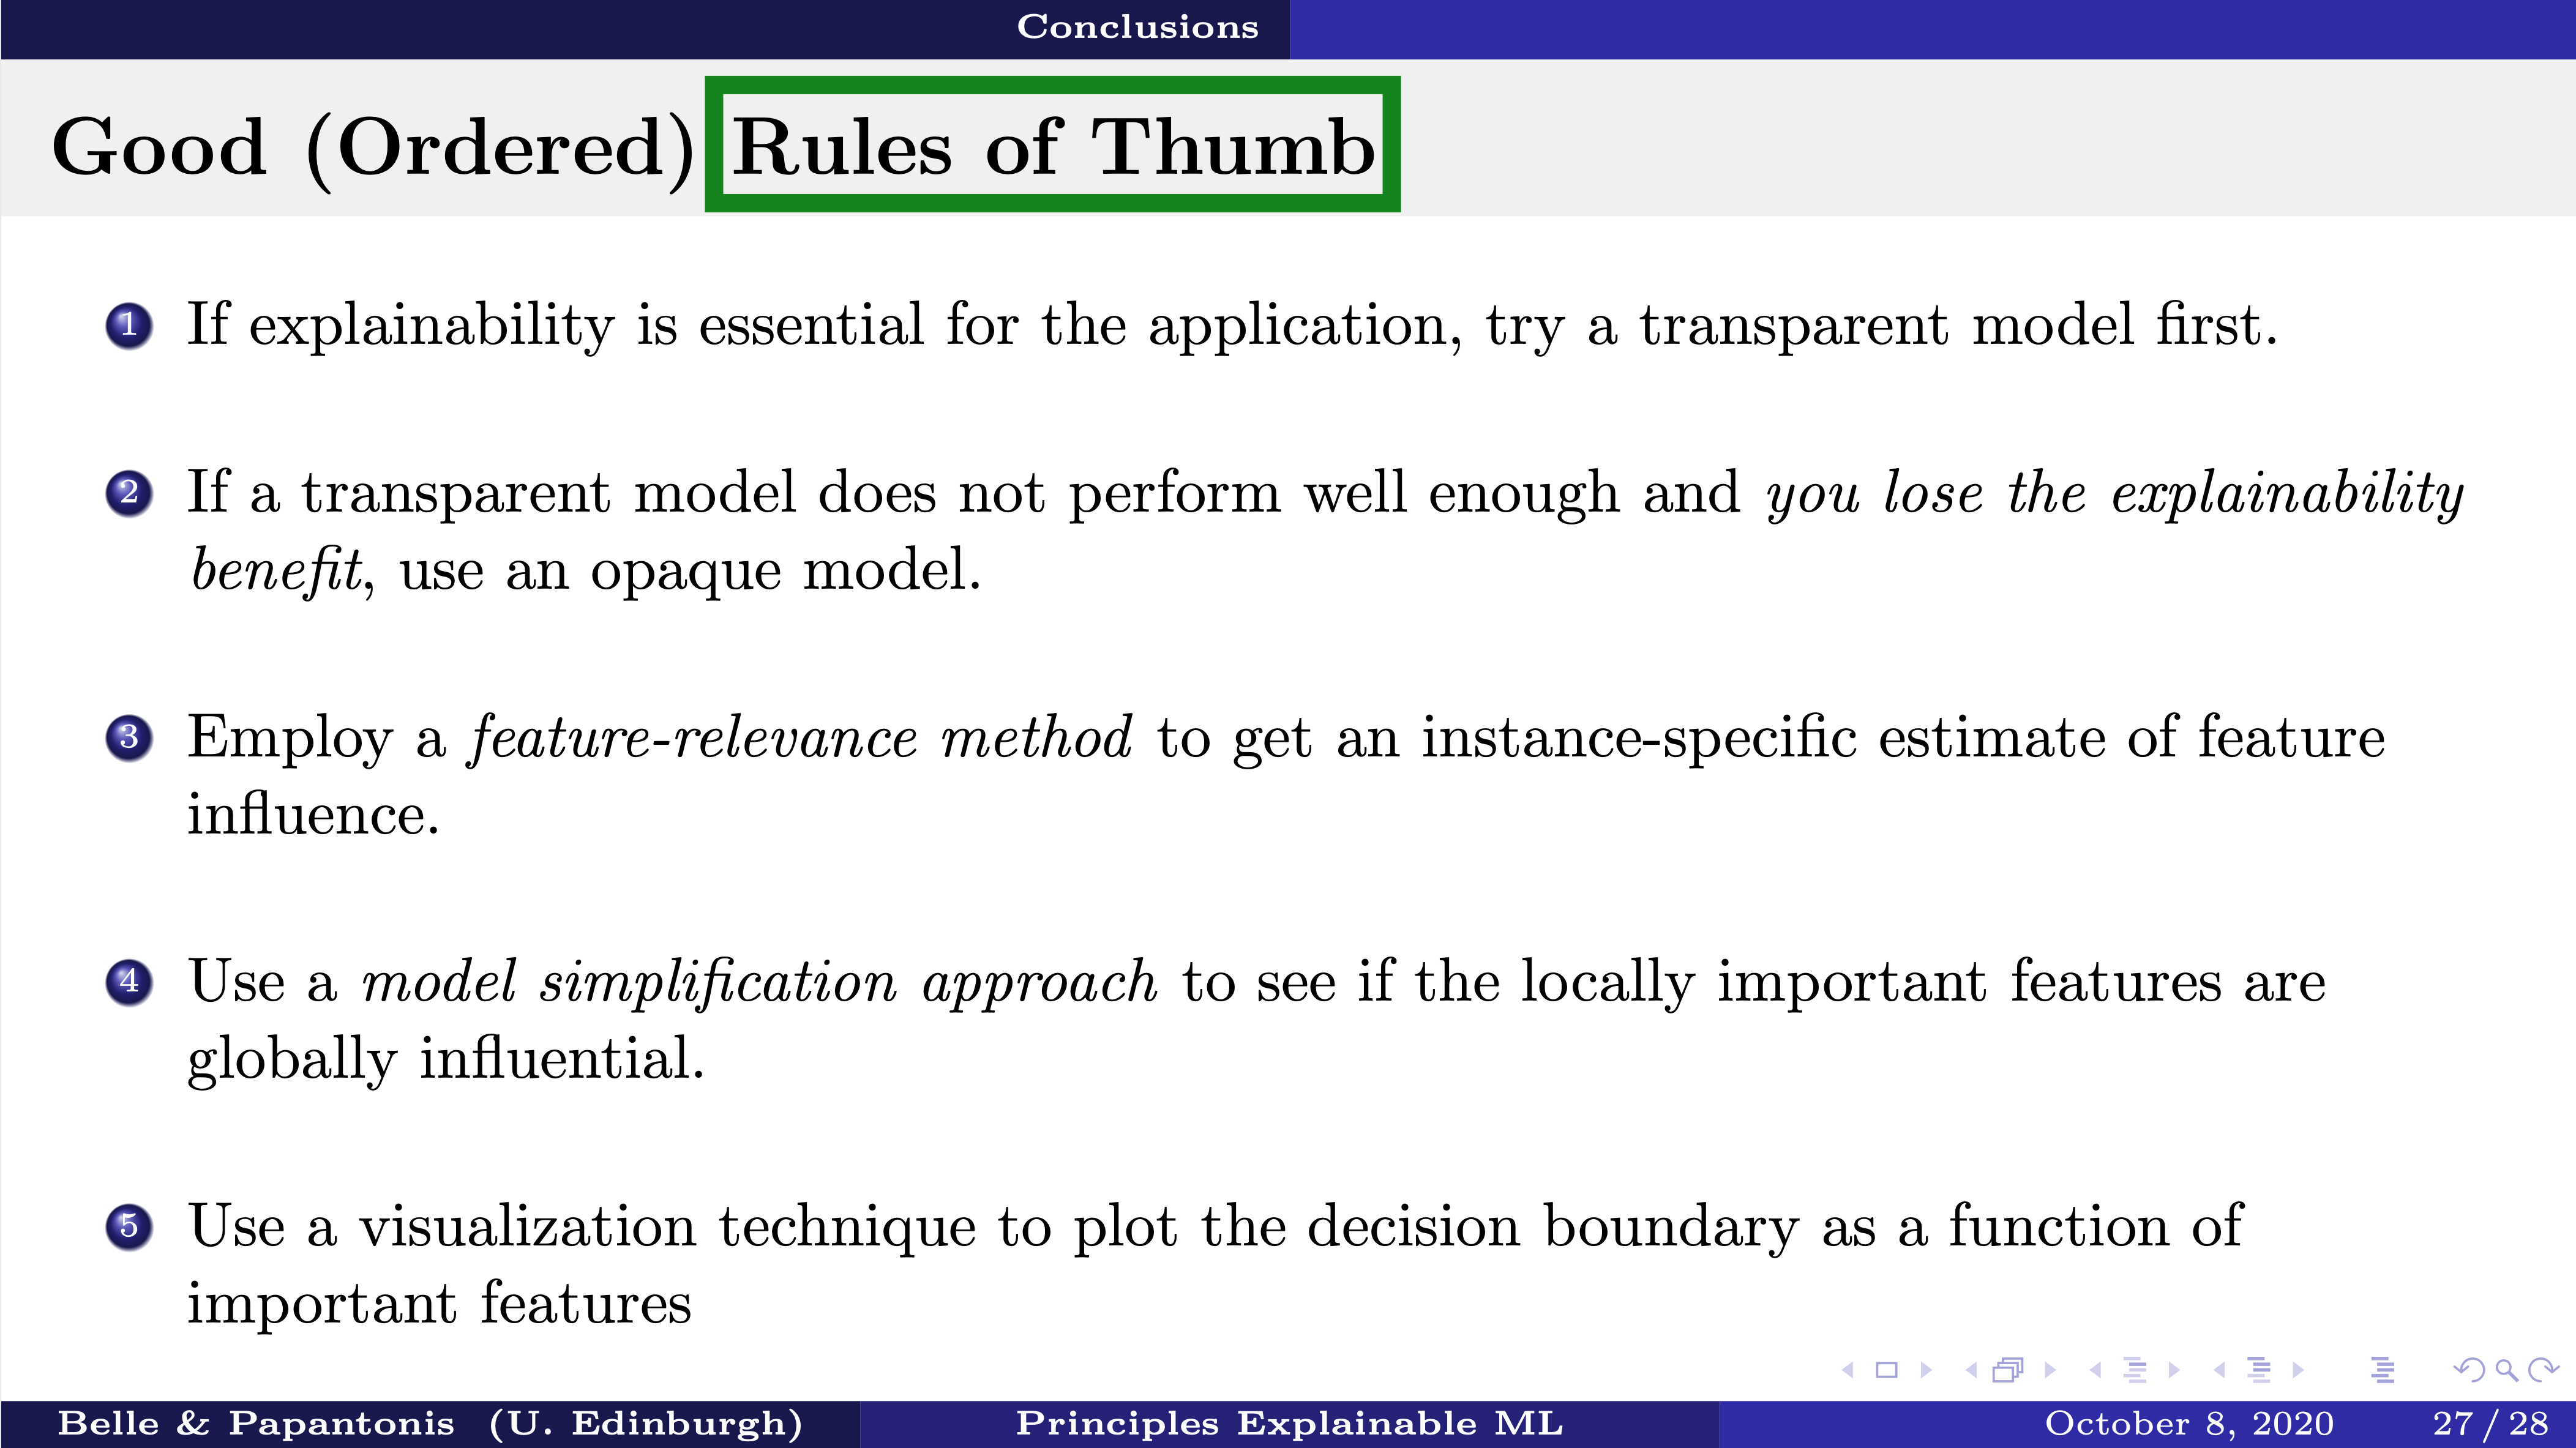
\includegraphics[scale=0.15]{rule_of_thumb_pres.png}
  \end{center}
\end{frame}

\begin{frame}{Week 5 Discussion on Canvas}
  \textbf{Paper}: ``Manipulating and Measuring Model Interpretability''~\citep{PoursabziSangdeh:2018} \\
  \textbf{Date}: October~29, 2020

  \vspace{12pt}
  ``I would summarize a \green{rule of thumb} for this as for most cases, combining `man and machine' was a bad idea.''
\end{frame}

\begin{frame}{What is a Rule of Thumb \& Why am I Obsessed with Them?}
  \textbf{Standard Definition}:
  \begin{itemize}
    \item Broadly but not strictly accurate
    \item Based on experience or practice rather than theory
  \end{itemize}

  \vspace{20pt}
    \onslide<2->{\textbf{Wikipedia Criteria}: ``easily learned and easily applied procedure''
    \begin{itemize}
      \item You might say ``short and sweet''
    \end{itemize}
  }
\end{frame}

\subsection{LIME}

\begin{frame}{LIME is a Bit \textit{Sour}}
  \blue{\textbf{LIME}}: Local Interpretable Model-Agnostic Explanations~\citep{Ribeiro:2016}
  \begin{itemize}
    \item \textbf{Authors}: Marco Tulio Ribeiro, Sameer Singh, \& Carlos Guestrin
  \end{itemize}

  \vspace{20pt}
  \textbf{\green{Similarity with Rules of Thumb}}
  \begin{itemize}
    \item Model-agnostic $\to$ Broadly applicable
  \end{itemize}

  \onslide<+->{
    \vspace{20pt}
    \textbf{\red{Disadvantages vs.\ Rules of Thumb}: What do you think?}
    \begin{itemize}[<+->]
      \item Linear model ${\stackrel{\mathclap{\mbox{\footnotesize \textnormal{?}}}}{\to}}$ Easily applied
      \item Local explanation $\not\to$ Broadly applicable
    \end{itemize}
  }
\end{frame}

\section{Anchors}
\subsection{Intuition}
\begin{frame}{Let's Build an Intuition First\ldots}
  \textbf{\blue{Task}}: Sentiment Analysis

  \vspace{2pt}
  \textbf{Representation}: Bag of words

  \vspace{8pt}
  \begin{center}
    \onslide<2->{
\includegraphics[scale=0.2]{sentiment_instances.png}}
  \end{center}

  \vspace{10pt}
  \begin{columns}
    \begin{column}{0.5\textwidth}
      \begin{center}
        \onslide<3->{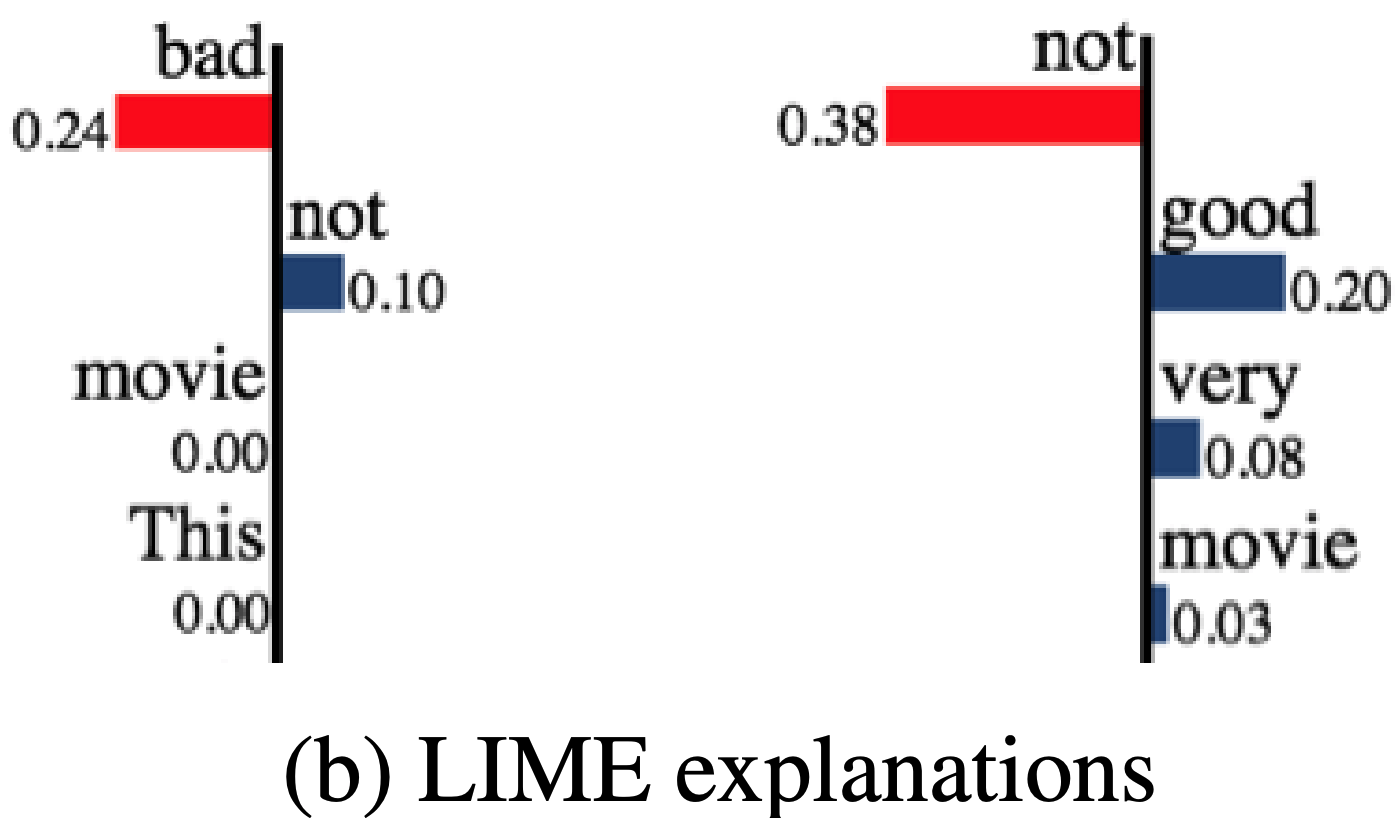
\includegraphics[scale=0.2]{sentiment_lime.png}}
      \end{center}
    \end{column}
    \begin{column}{0.5\textwidth}
      \begin{center}
        \onslide<4->{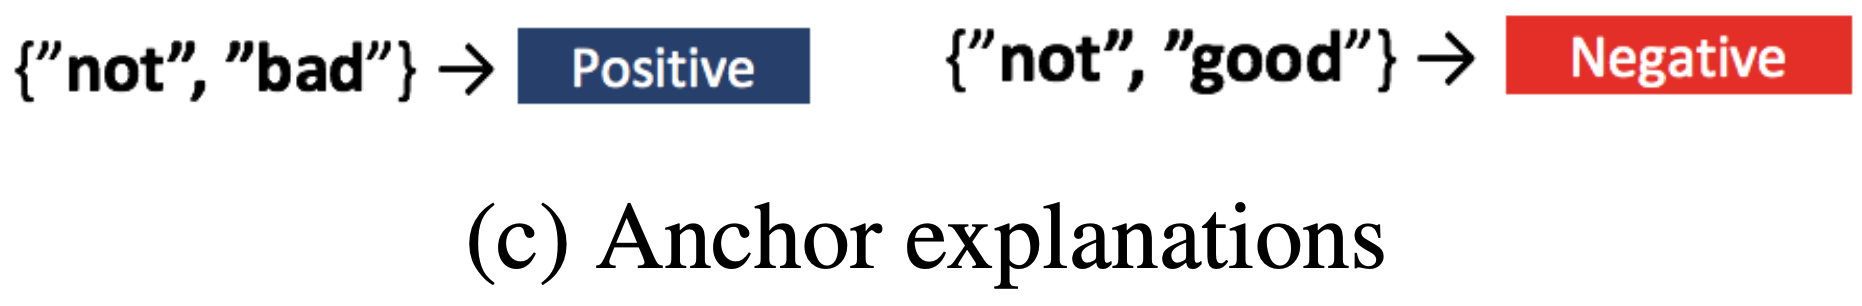
\includegraphics[scale=0.2]{sentiment_anchors.png}}
      \end{center}
    \end{column}
  \end{columns}
\end{frame}

\begin{frame}{Anchors are Just Rules of Thumb}
  \noindent
  \textbf{Proposed By}: Marco Tulio Ribeiro, Sameer Singh, \& Carlos Guestrin (sound familiar?)

  \vspace{20pt}
  \noindent
  \onslide<+->{\green{\textbf{Anchors Features vs.\ Rules of Thumb}}: What are the similarities?}
  \begin{itemize}[<+->]
    \item Model-agnostic $\to$ Broadly applicable
    \item Global explanation $\to$ Broadly applicable
    \item Compact if-then rules $\to$ Easily applied
    \item Accurate: Let's get back to this in a bit\ldots
  \end{itemize}
\end{frame}

\subsection{Definition}
\begin{frame}{Definition}
  \onslide<+->{}
  \begin{block}{Anchor}
    Explanation that \textit{sufficiently} explains the \textit{model} behavior
  \end{block}

  \vspace{15pt}
  \onslide<+->{%
    \textbf{\blue{Question}}: What does \textit{sufficiency} imply here?

    \vspace{10pt}
    \onslide<+->{\textbf{Answer}: If the rule holds, nothing else (e.g.,~features) matters.}

    \vspace{10pt}
    \begin{itemize}[<+->]
      \item That's a \textbf{\green{big deal}}!  Goes even further than rules of thumb\ldots
    \end{itemize}
  }
\end{frame}

\begin{frame}{Let's Get Technical: Part~1}
  \onslide<+->{\textbf{Two New Metrics}: \textbf{\blue{Precision}} \& \textbf{\blue{Coverage}}}

  \vspace{16pt}
  \onslide<+->{\textbf{\blue{Precision}}: What is the definition?

    \vspace{4pt}
    \onslide<+->{%\textbf{Standard Definition}:
      \begin{equation}
        \xxcancel<+->{\text{Precision} \defeq \frac{TP}{TP + FP}}
      \end{equation}
    }

    \vspace{12pt}
    \onslide<+->{\textbf{\blue{Question~\#1}}: What is an intuitive explanation for why this definition is wrong?}

    \vspace{6pt}
    \onslide<+->{\textbf{Answer}: Reality (labels) is \textbf{\red{not}} ground-truth. The \textbf{\green{model}} is now \textit{truth}!}

    \vspace{18pt}
    \onslide<+->{\textbf{\blue{Question~\#2}}: Why are we using precision and not accuracy?}
  }
\end{frame}

\begin{frame}{Let's Get Technical: Part~2}
  \textbf{Two New Metrics}: \textbf{\blue{Precision}} \& \textbf{\blue{Coverage}}

  \vspace{20pt}
  \onslide<+->{\textbf{\blue{Coverage}}: What is the definition?

    \vspace{10pt}
    \onslide<+->{%\textbf{Standard Definition}:
      Extent (e.g.,~fraction of examples) to which the rule applies
    }

    \vspace{20pt}
    \onslide<+->{Unlike LIME, coverage of an anchor is very clear.}
  }
\end{frame}

\begin{frame}{Mathematical Formulation}
  \begin{itemize}[<+->]
    \setlength{\itemsep}{10pt}
    \item $\func{\dec}{\domainX}{\domainY}$: Decision function
    \item $\func{\Rule}{\domainX}{\set{0,1}}$: \underline{A}nchor rule
    \item ${\Rule \in \setRule}$: Set of rules
    \item ${\dist(\cdot \vert \Rule)}$: Conditional probability distribution conditioned on rule
    \item ${\minPrec \in [0,1]}$: Minimum anchor accuracy probability
    \item \blue{Precision}:
      \begin{equation}
        \Prec{A} \defeq \expectS{z \sim \dist(\cdot \vert \Rule)}{\ind{\dec(x) = \dec(z)}}
      \end{equation}
    \item \blue{Coverage}:
      \begin{equation}
        \cov{A} \defeq \expectS{z \sim \dist(\cdot)}{A(z)}
      \end{equation}
  \end{itemize}
\end{frame}

\subsection{Examples}

\begin{frame}{Visualizing the Mathematical Formulation}
  \begin{columns}
    \begin{column}{0.33\textwidth}
      \onslide<+->{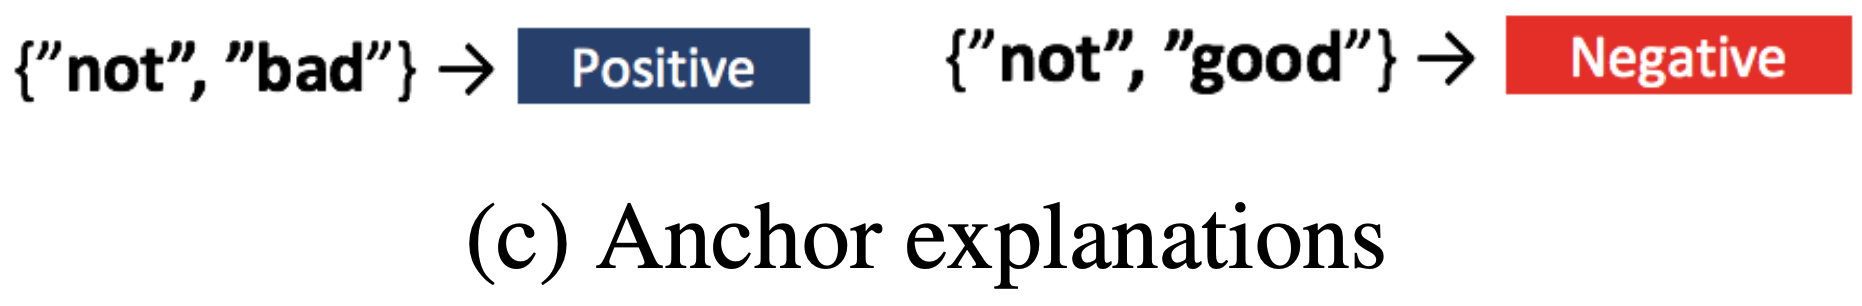
\includegraphics[scale=0.15]{sentiment_anchors.png}}
    \end{column}
    \begin{column}{0.33\textwidth}
      \begin{center}
        \onslide<+->{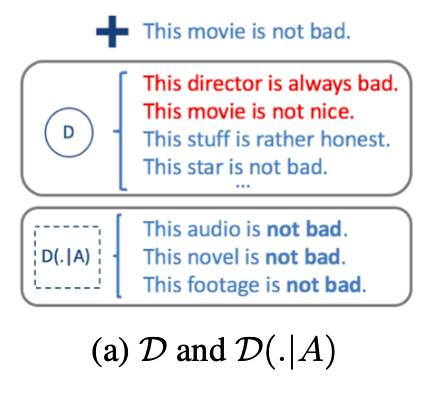
\includegraphics[scale=0.3]{dist_ex.png}}
      \end{center}
    \end{column}
    \begin{column}{0.33\textwidth}
      \begin{center}
        \onslide<+->{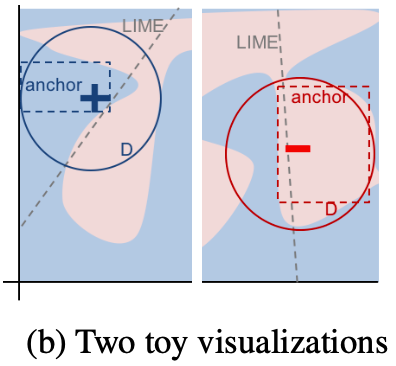
\includegraphics[scale=0.3]{anchor_visualization.png}

          \vspace{20pt}
          Highly non-linear
        }
      \end{center}
    \end{column}
  \end{columns}
\end{frame}

\begin{frame}{Example: Structured Prediction}
  \begin{center}
    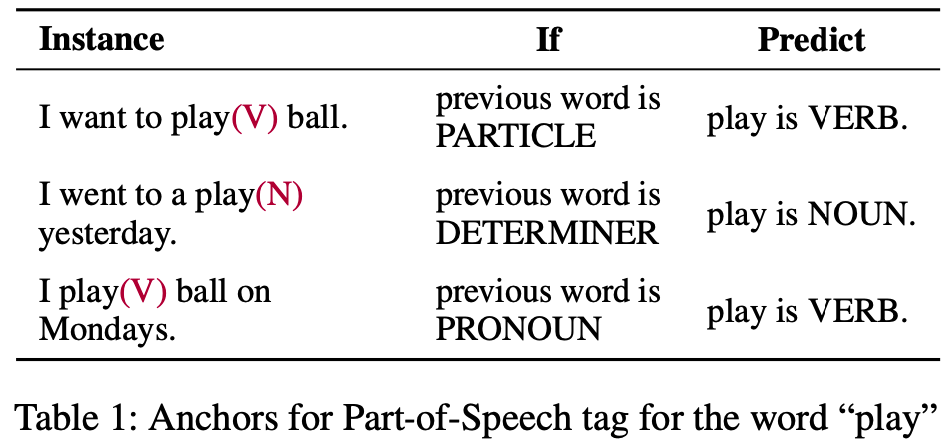
\includegraphics[scale=0.4]{structured_ex.png}
  \end{center}
\end{frame}

\begin{frame}{Example: Tabular Data}
  \begin{center}
    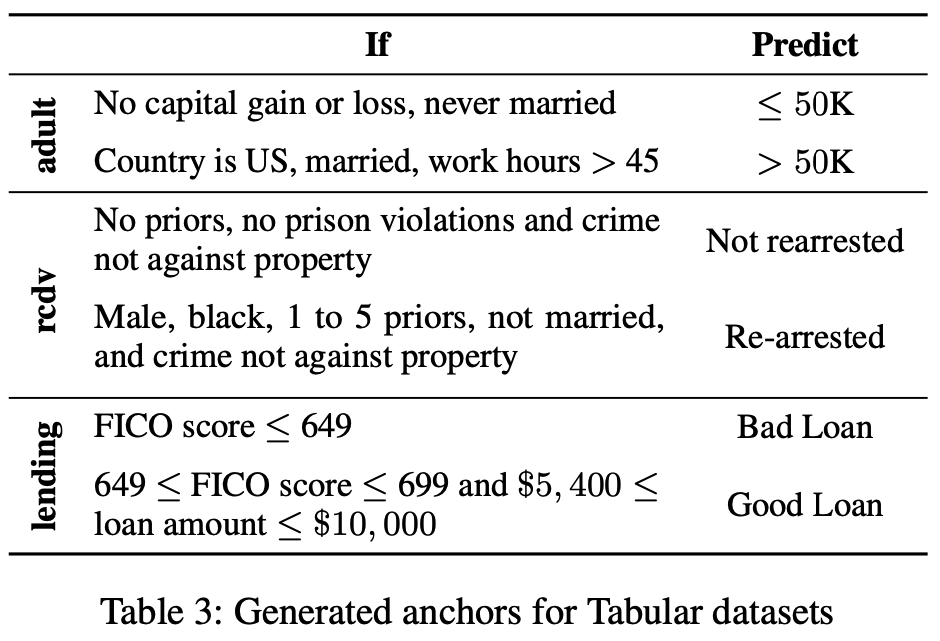
\includegraphics[scale=0.3]{tabular_ex.png}
  \end{center}
\end{frame}

\begin{frame}{Example: Visual Question \& Answer (VQA)}
  \begin{center}
    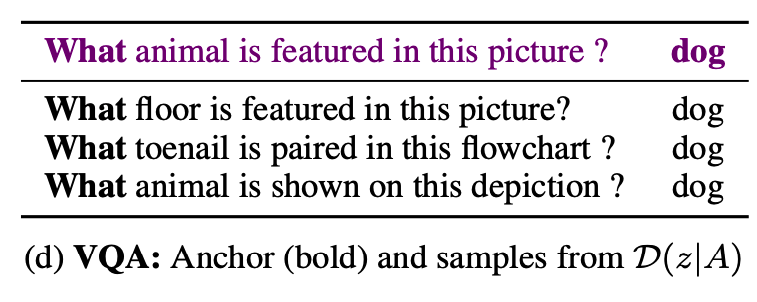
\includegraphics[scale=0.4]{vqa_ex.png}
  \end{center}
\end{frame}

\section{Efficiently Computing Anchors}

\begin{frame}{Relaxing the Formulation: \textbf{\blue{Precision}}}
  % \onslide<+->{%
    % \blue{Precision}:
    \begin{equation}
      \Prec{A} \defeq \expectS{z \sim \dist(\cdot \vert \Rule)}{\ind{\dec(x) = \dec(z)}} \onslide<2->{ \geq \minPrec}
    \end{equation}
    % \vspace{6pt}
    \onslide<2->{Authors used ${\minPrec = 0.95}$}

    \vspace{15pt}
    \onslide<3->{In almost all cases, ${\dist(z \vert \Rule)}$ is unknown in practice.}

    \vspace{15pt}
    \onslide<4->{
      Relaxed formulation:
      \begin{equation}
        \Pr \sbrack{\Prec{A} \geq \minPrec} \geq 1 - \delta \text{.}
      \end{equation}
    }

    \onslide<5->{\textbf{Question}: What mathematical formulation is commonly used in practice to guarantee these bounds?}
  % }
%   \vspace{20pt}
%   \onslide<+->{%
%     \blue{Coverage}:
%     \begin{equation}
%       \cov{A} \defeq \expectS{z \sim \dist(\cdot)}{A(z)}
%     \end{equation}
%   }
\end{frame}

\begin{frame}{Relaxing the Formulation: \textbf{\blue{Coverage}}}
  Given a set of Anchors with \textit{acceptable} precision, we seek rules with the best coverage.  Recall the definition of coverage:
  \begin{equation}
    \cov{A} \defeq \expectS{z \sim \dist(\cdot)}{A(z)}
  \end{equation}

  \vspace{20pt}
  \onslide<2->{Combinatorial optimization problem:
    \begin{equation}
      \max_{\Rule \text{ s.t. } \Pr\sbrack{\Prec{A} \geq \minPrec} \geq 1 - \delta} \cov{A}
    \end{equation}

    \vspace{10pt}
    Although not an explicit constraint, greater coverage implicitly favors simpler rules.
  }
\end{frame}

\subsection{Greedy}
\begin{frame}{Greedy Algorithm}
  \begin{columns}
    \begin{column}{0.5\textwidth}
      I found the authors' explanation here a bit lacking.  I believe I have determined their main idea.
      \begin{itemize}
        \item If something is missing/off-base here, feel free to jump in.
      \end{itemize}

      \onslide<2->{%
        \vspace{10pt}
        \begin{itemize}
          \item $\predicate_{i}$: Predicate, i.e.,~binary test
        \end{itemize}

        \vspace{10pt}
        Function \textsc{GenerateCands} exhaustively constructs all \textit{combinations} of predicates with sufficient coverage~${{>}\minCov}$
      }
    \end{column}
    \begin{column}{0.5\textwidth}
      \begin{center}
        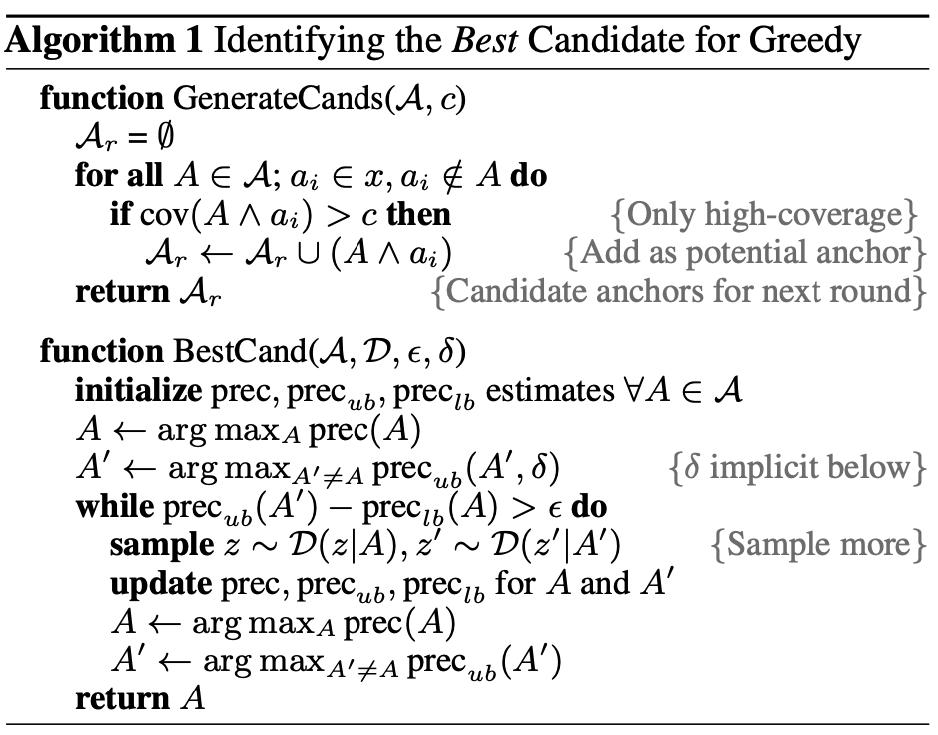
\includegraphics[scale=0.20]{alg_greedy.png}
      \end{center}
    \end{column}
  \end{columns}
\end{frame}

\subsection{Beam Search}
\begin{frame}{Beam Search Algorithm}
  \begin{columns}
    \begin{column}{0.5\textwidth}
      \textbf{Beam Search}: A ``greatest-hit'' algorithm
      \begin{itemize}
        \item Useful to lots of domains
        \item $\beamWidth$: Beam width
      \end{itemize}

      \vspace{10pt}
      \textbf{\blue{Question}}: What are the differences between greedy and beam search?

      \vspace{10pt}
      \onslide<2->{\textbf{\blue{Question}}: How does the computational complexity compare?}
    \end{column}
    \begin{column}{0.5\textwidth}
      \begin{center}
        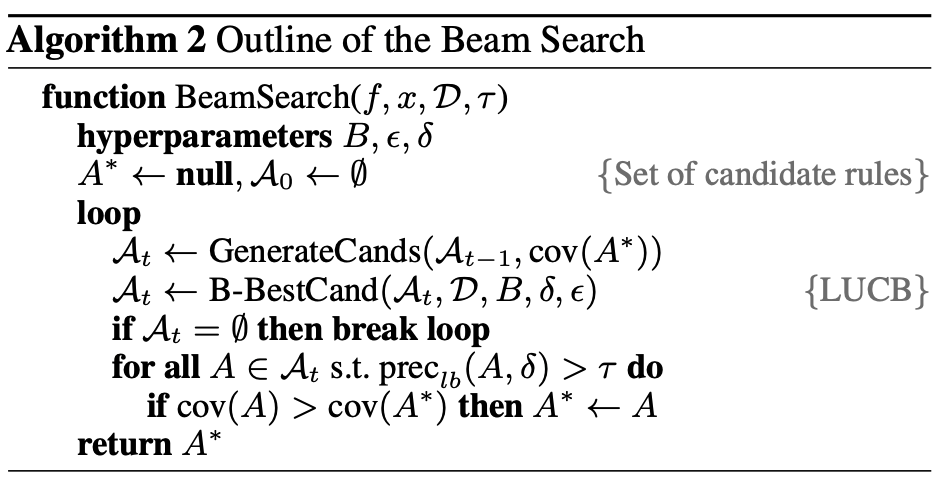
\includegraphics[scale=0.225]{alg_beam_search.png}
      \end{center}
    \end{column}
  \end{columns}
\end{frame}

\section{User Study}

\begin{frame}{A Well-Done User Study}
  \begin{itemize}
    \setlength{\itemsep}{12pt}
    \item \textbf{Focus Group}: 26~students in a machine learning course
    \item \textbf{Three Datasets}: \texttt{adult}, \texttt{rcdv}, and \texttt{vqa}
    \item Half see a LIME first and Anchors second
      \begin{itemize}
        \item Vice versa for the other half
      \end{itemize}
    \item \textbf{Metrics}: Precision, Coverage, \& Prediction time
      \begin{itemize}[<+->]
        \item \textbf{I Don't Know}\ldots: Coverage \& precision calculated \red{\textbf{only}} from examples where user made a prediction other than ``I don't know''
        \item This is why \textit{accuracy} is an inappropriate metric
      \end{itemize}
    \item LIME \& Anchors: Explanations of similar size
  \end{itemize}
\end{frame}

\begin{frame}{User Study Results}
  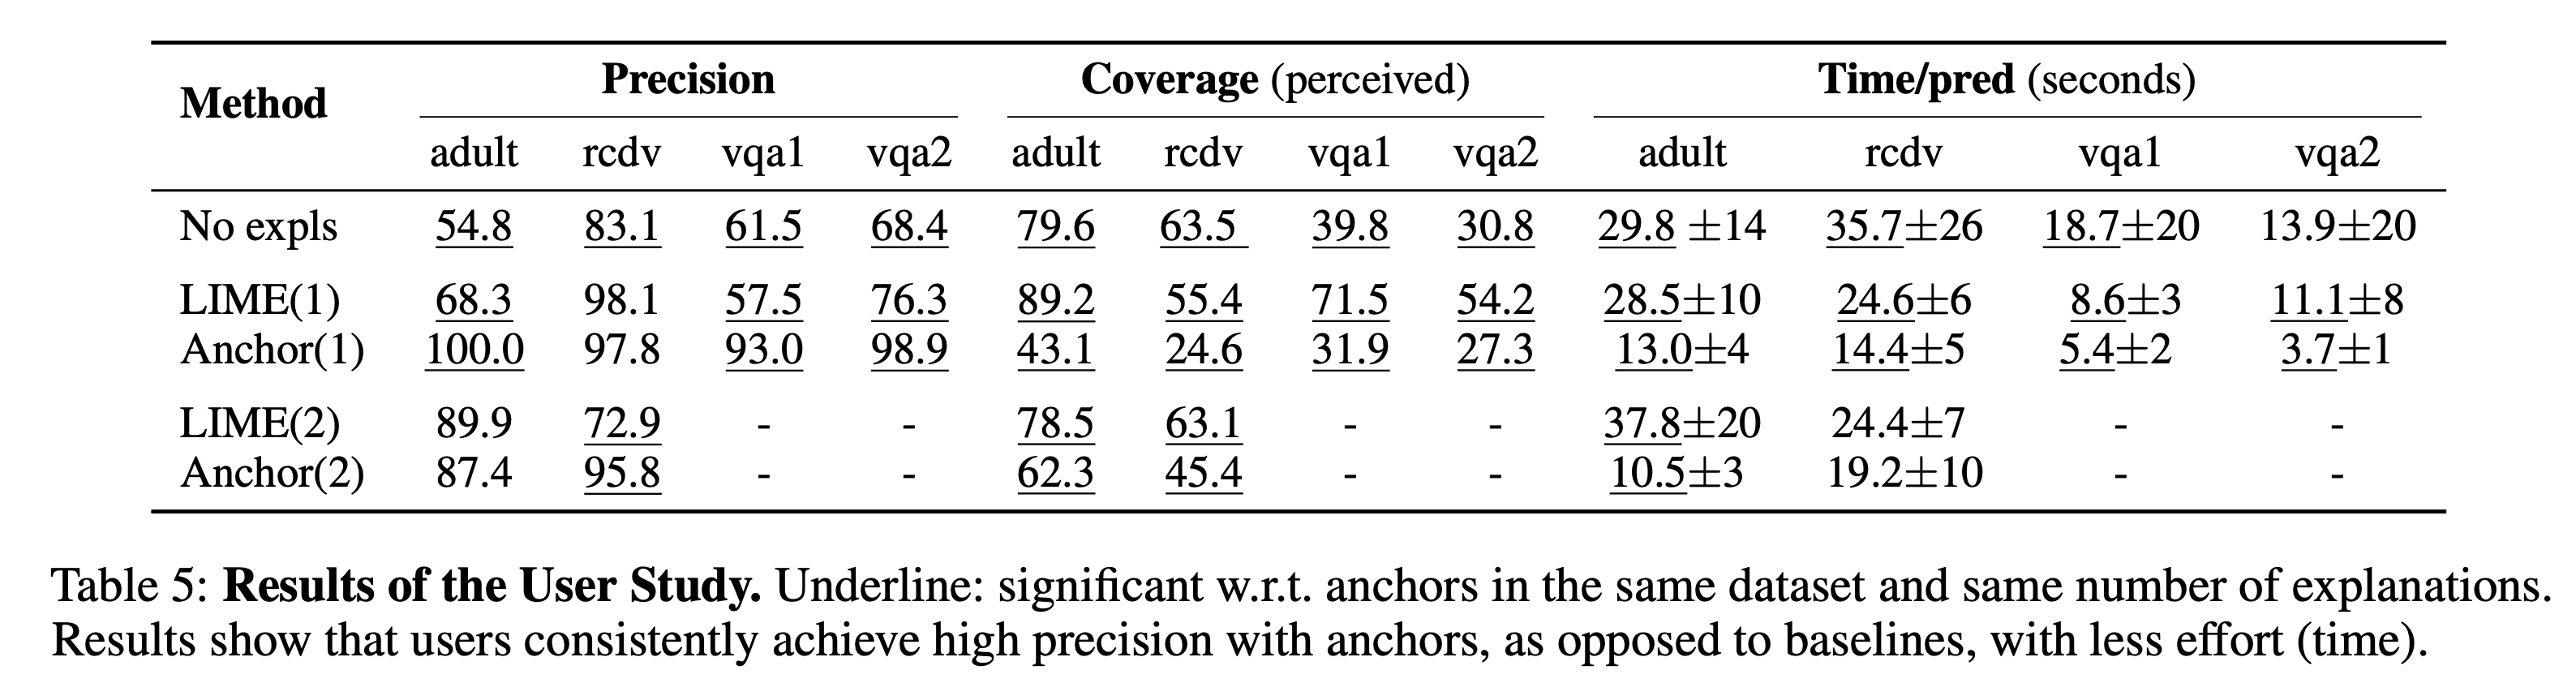
\includegraphics[scale=0.25]{img/user_study.png}

  \begin{center}
    It may be easier to read if you use a local copy of the table
  \end{center}
\end{frame}

\begin{frame}{Always Have a Survey}
  Counter-intuitive results always have a big impact on reviewers/readers\ldots
  \begin{itemize}
    \setlength{\itemsep}{10pt}
    \item 21/26 preferred Anchors
    \item 24/26 felt they were more precise with Anchors
      \begin{itemize}
        \item The 2 who felt more precise with LIME were \textit{actually} more precise with Anchors
      \end{itemize}
  \end{itemize}
\end{frame}

\section{Limitations}

\begin{frame}{Conflicting Anchors}
  \textbf{\blue{Basic Idea So Far}}: If anchor rule applies, trust its prediction.

  \vspace{15pt}
  This could happen for a couple of reasons\ldots
  \begin{itemize}
    \item Anchors's probabilistic nature makes that inevitable
    \item Submodular objective encourages low-overlap rules
  \end{itemize}

  \vspace{15pt}
  \textbf{\blue{Question}}: What is the best solution?

  \onslide<2->{\vspace{6pt}
    \textbf{Answer}: Not obvious.  Perhaps all you can do is alert the user of the conflict and let them sort it out
  }
\end{frame}

\begin{frame}{Graphical Explanations}
  \textbf{Note}: This is my own perspective and not from the paper itself.

  \begin{columns}
    \begin{column}{0.5\textwidth}
      \begin{center}
        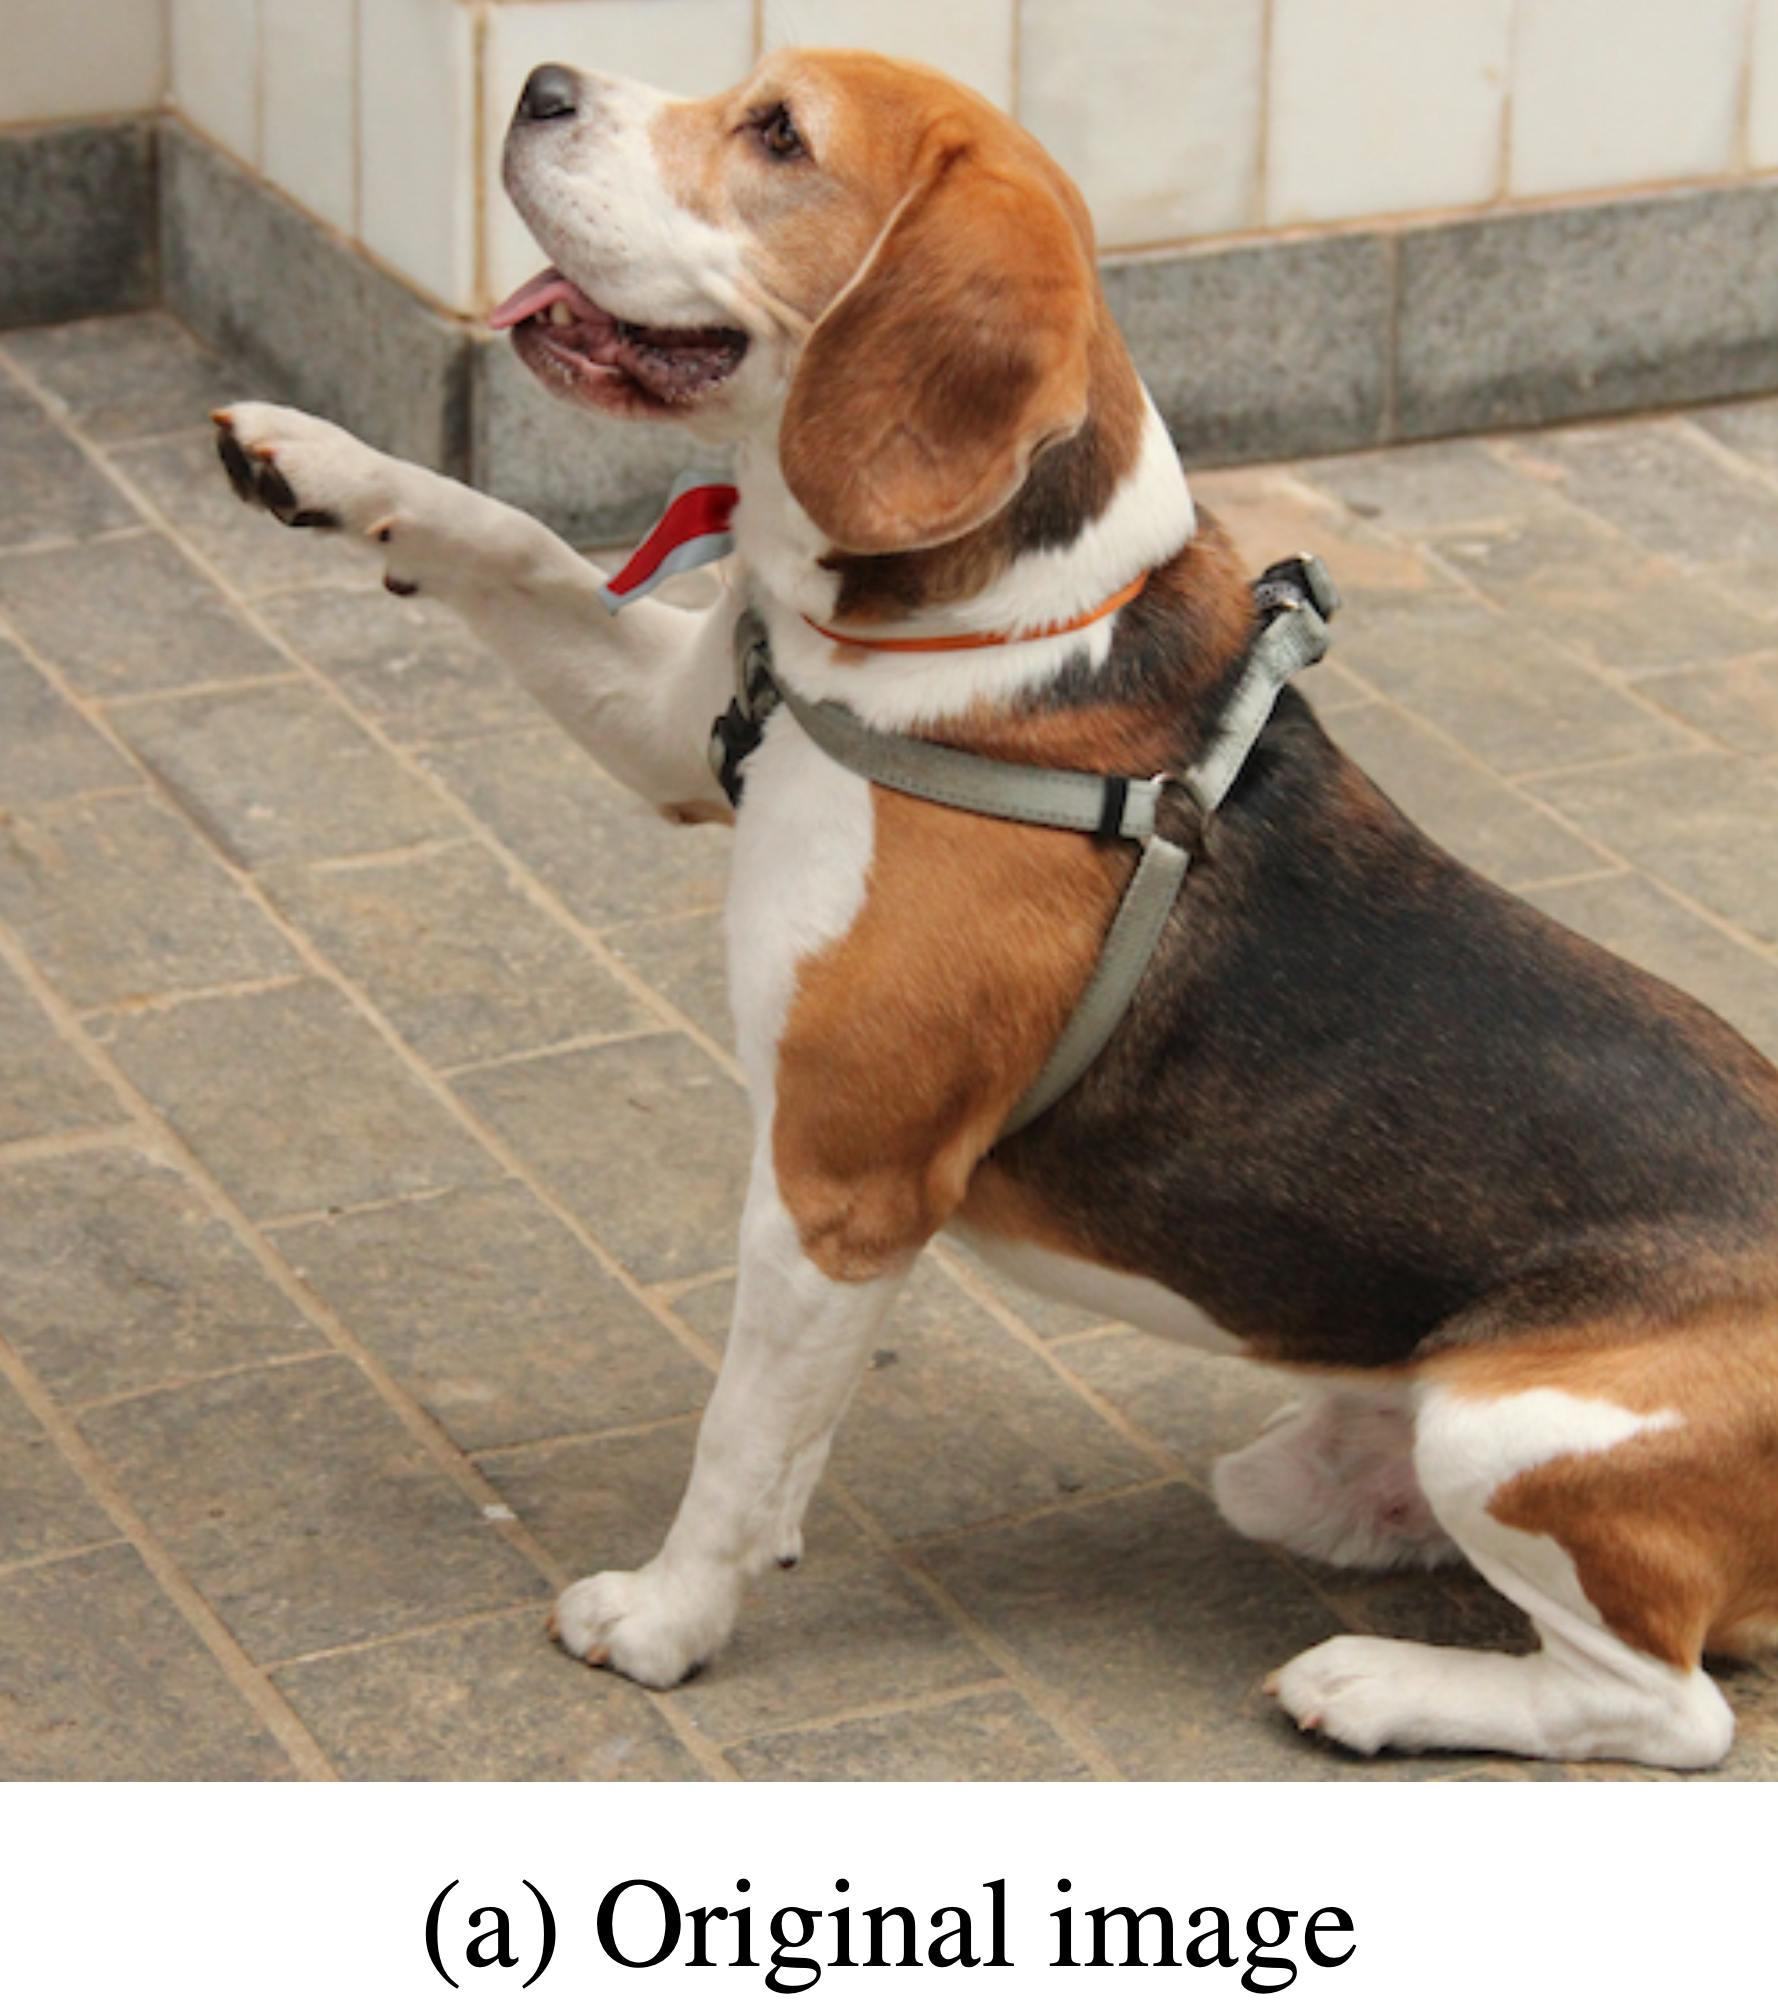
\includegraphics[scale=0.09]{beagle_original.png}
      \end{center}
    \end{column}
    \begin{column}{0.5\textwidth}
      \begin{center}
        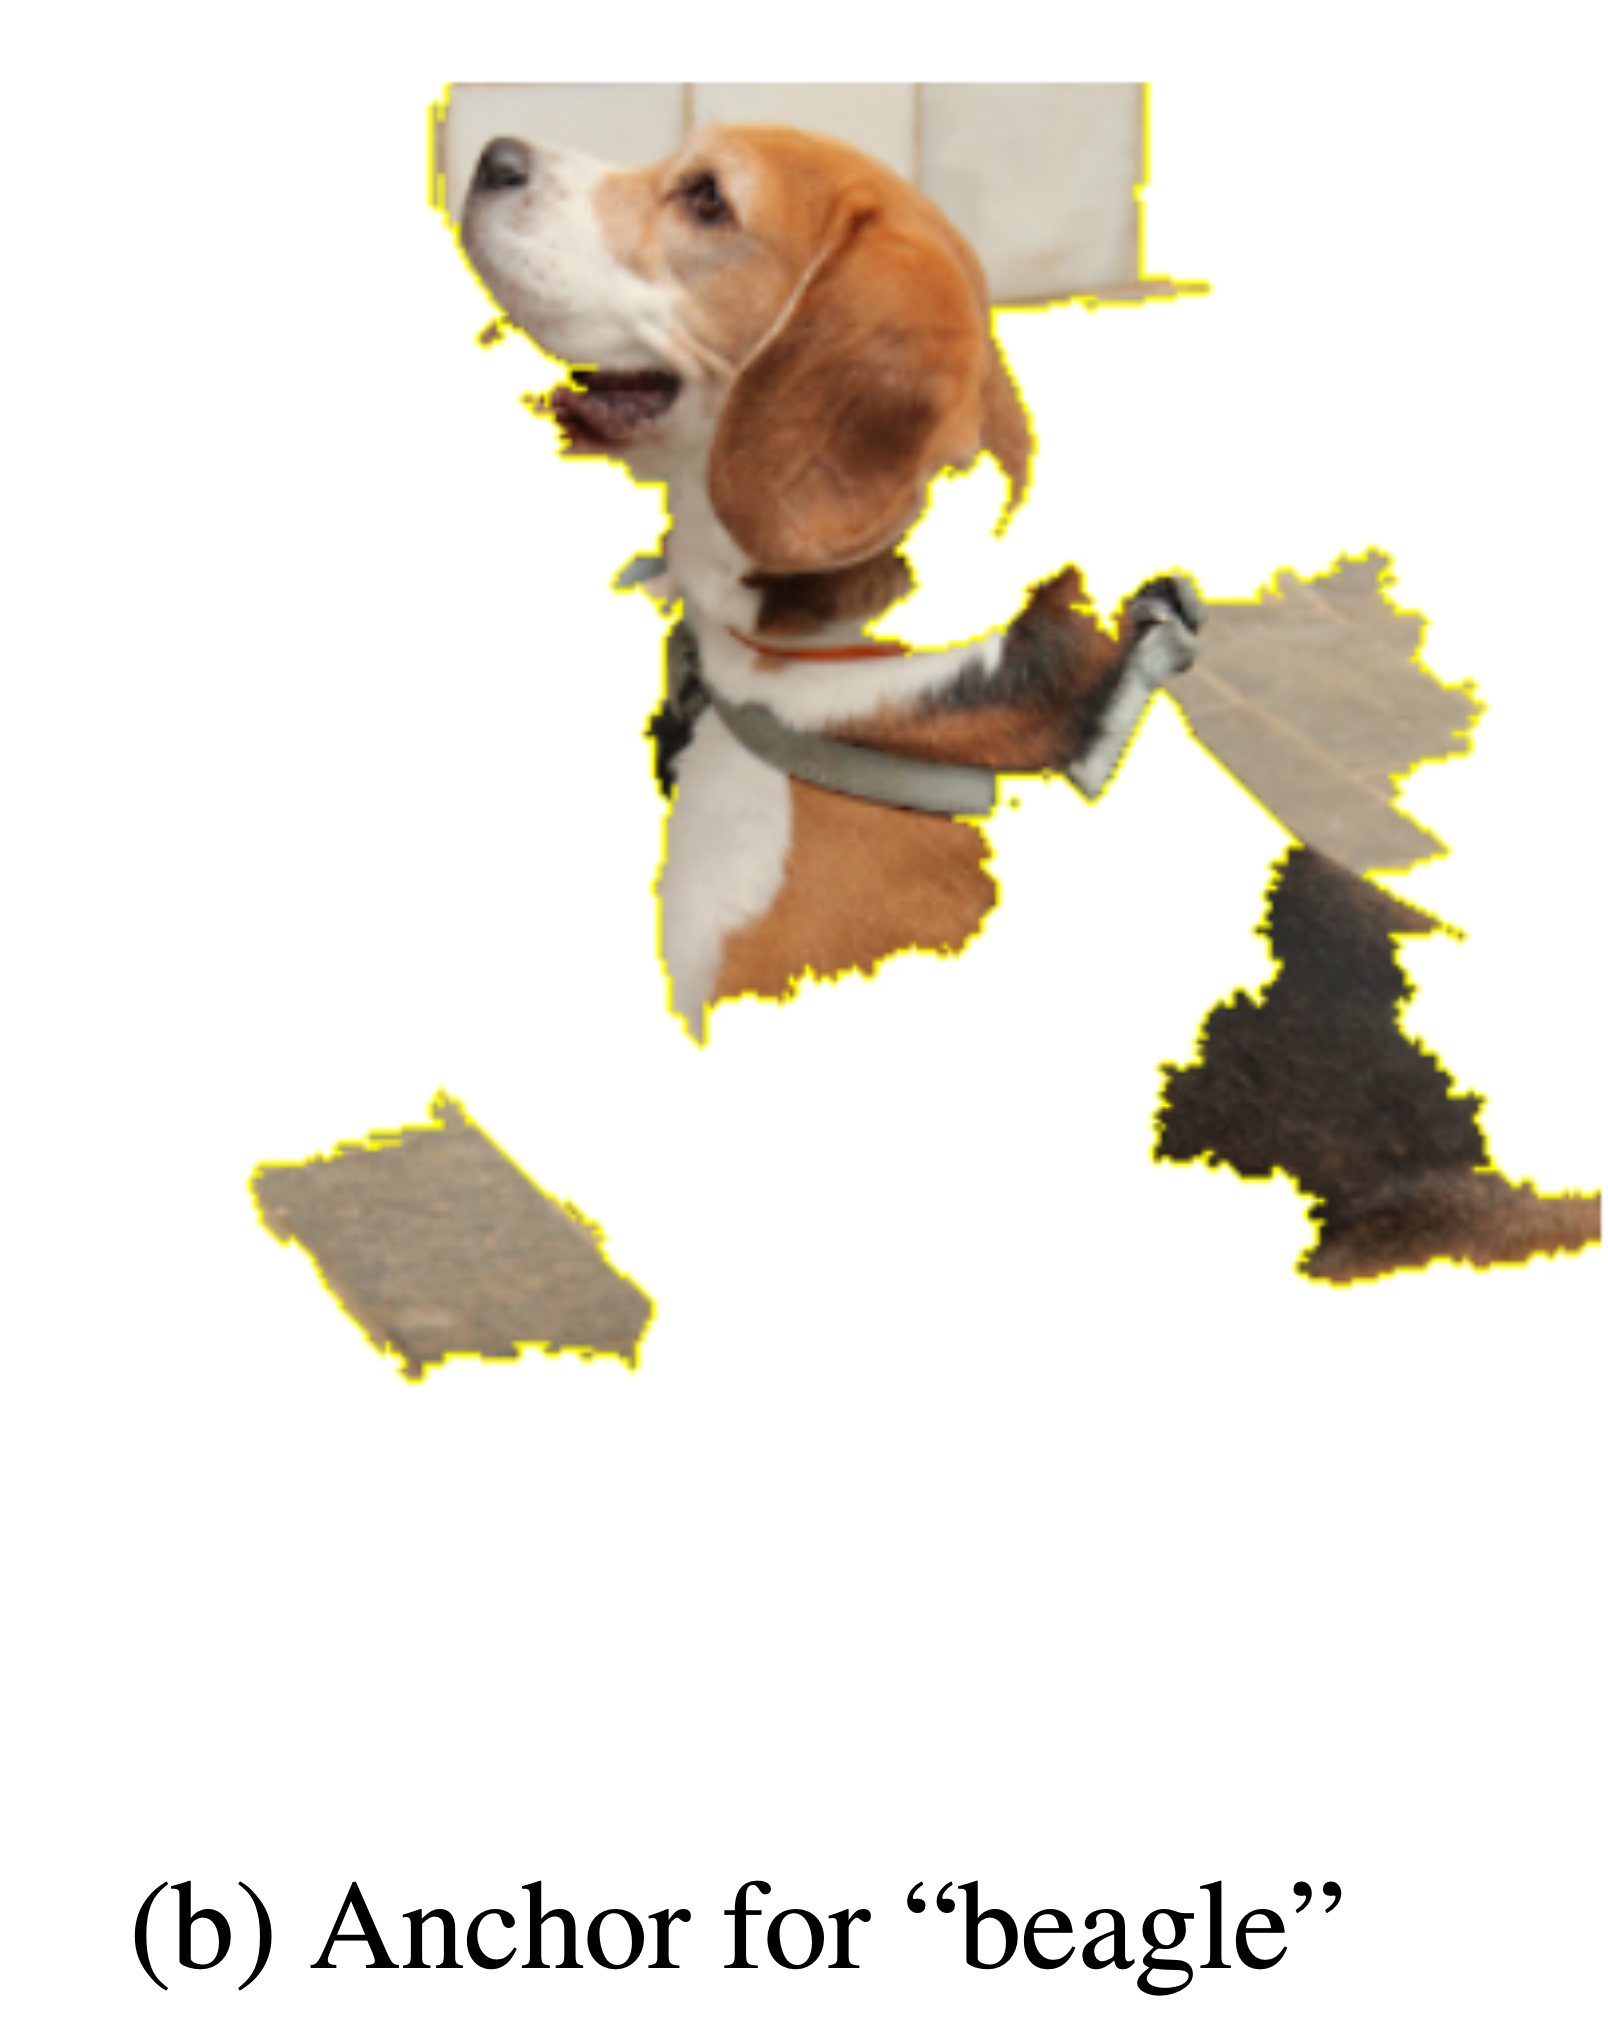
\includegraphics[scale=0.09]{beagle_anchor.png}
      \end{center}
    \end{column}
  \end{columns}

  \vspace{15pt}
  \textbf{\blue{Question}}: Is this \textit{anchor} meaningful?

  \vspace{6pt}
  \onslide<2->{I would argue \textbf{\red{no}} since rule does not generalize.  It is essentially a local explanation.}

  \vspace{6pt}
  \onslide<3->{With NLP~models increasingly requiring contextual embeddings, do we have the same problem with text too?}
\end{frame}

\begin{frame}[noframenumbering]{Table of Contents}
  \tableofcontents
\end{frame}

\begin{frame}[noframenumbering,allowframebreaks]{Bibliography}{}
  {\tiny
    \frametitle{References}
    \bibliography{bib/ref.bib}
    \bibliographystyle{unsrtnat}
  }
\end{frame}

\begin{frame}{Talking Points: Greedy}
  \begin{itemize}
    \setlength{\itemsep}{8pt}
    \item What is an intuitive explanation of multi-armed bandit?
    \item What is the definition of \textbf{\blue{estimation error}} in machine learning theory?
    \item What is an \textbf{intuitive} understanding of Eq.~(5)?
  \end{itemize}
\end{frame}
\end{document}
